\documentclass{cumcmthesis}
\usepackage[framemethod=TikZ]{mdframed}
\usepackage{url}   % 网页链接
\usepackage{subcaption} % 子标题
\usepackage{tikz}
\usetikzlibrary{shapes.geometric, arrows.meta, positioning, fit}
\usetikzlibrary{positioning,arrows.meta,calc}
% Avoid hyperref warnings about tokens in PDF strings (from xeCJK/ctex internals)
\makeatletter
\pdfstringdefDisableCommands{%
    \def\leavevmode{}%
    \def\leavevmode@ifvmode{}%
    \def\kern#1{}%
}
\makeatother
% Improve PDF bookmark handling and encoding for hyperref
\usepackage{bookmark}
\hypersetup{unicode=true, pdfencoding=auto}

\title{智能制造场景零件的智能检测及无序分拣}

% 提供安全日期格式,避免类里对日期的特殊宏(如 \mon)未定义导致报错
\author{作者姓名}
\date{\today}

 
\begin{document}
\newpage
% Minimal document body to avoid Emergency stop during compilation
\begin{abstract}
随着智能制造的发展,工件检测和缺陷识别在工业生产中变得越来越重要。传统的人工检测方法效率低且易受主观因素影响,难以满足现代制造业对高效、精准检测的需求。
本文首先提出了基于计算机视觉的工件检测方案,利用深度学习技术实现对工件表面缺陷的自动识别。其次,设计了一套无序分拣系统,通过图像处理和机器学习算法,实现对不同类型工件的分类和分拣。最后,通过实验验证了所提方案的有效性和实用性,结果表明该系统在提高检测效率和准确率方面具有显著优势。
\keywords{工件检测, 缺陷识别, 计算机视觉, 深度学习}
\end{abstract}

\section{项目背景与意义}

随着智能制造的快速发展,生产线正逐步向柔性化、无人化和高精度方向转型。传统制造业中,零部件的检测与分拣往往依赖人工操作,存在以下问题:

\begin{enumerate}
    \item \textbf{检测精度不稳定:} 人工检测容易受主观因素影响,对细微划痕、脏污等缺陷识别准确率低。
    \item \textbf{劳动强度高、效率低:} 大量重复性检测与分拣工作占用了人力资源,生产节拍难以匹配自动化产线节奏。
    \item \textbf{零件种类多、形态复杂:} 以“三钢柱塞泵连杆配件原厂件泵头零件”为例,其具有多种型号(22/26/30/60/80/90/100/120),不同尺寸与表面反光特性导致传统视觉检测系统泛化能力不足。
    \item \textbf{无序堆放带来挑战:} 在制造环节中,零件常处于随机堆放状态,传统机械臂需人工摆放或依赖固定夹具,柔性差。
\end{enumerate}

基于此,本项目以“\textbf{智能制造场景下的零件智能检测及无序分拣系统}”为研究对象,聚焦于三钢柱塞泵系列零件的自动化检测与抓取,构建一套从缺陷识别到自主分拣的智能化系统。



该项目的研究与应用将提升制造业中零件检测与分拣环节的自动化水平,降低人工成本与误检率,推动智能制造向“感知—决策—执行”一体化方向发展,并为泵类零件等精密部件的质量控制提供智能化解决方案。
近年来,面向工业4.0的智能制造与云—边协同架构快速发展,推动产线数字化、柔性化升级\cite{lasi2014industry,shi2016edge,davis2015smart}。
\section{场景与系统总体架构}

本项目以“三钢柱塞泵连杆配件原厂件泵头零件”的生产与检测环节为研究对象,构建了一个面向智能制造场景的零件智能检测与无序分拣系统。系统整体由 \textbf{感知层、决策层、执行层} 三部分构成,涵盖了从图像采集、缺陷识别、抓取规划到机械臂执行的完整流程。

\subsection{场景描述}

\begin{figure}[htbp]
    \centering
    % 简化占位图以避免 calc/单位错误
    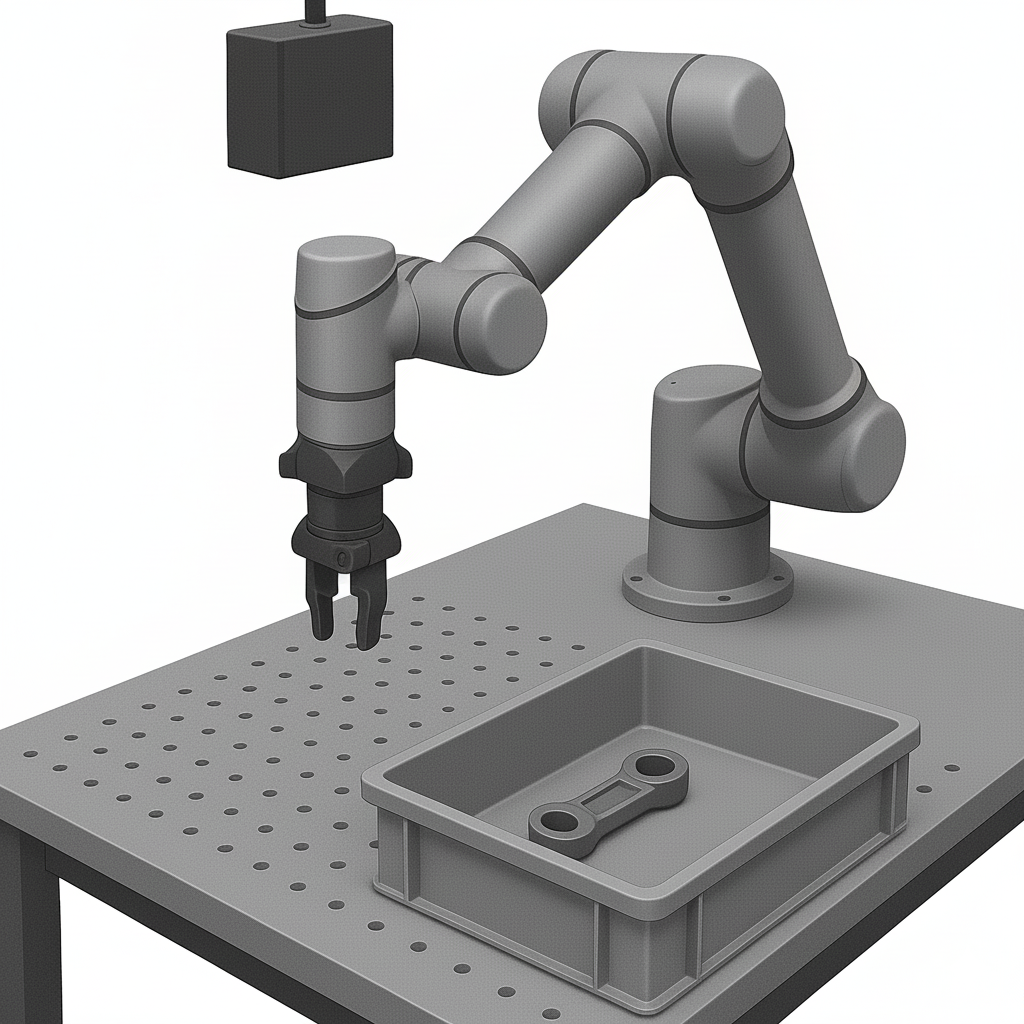
\includegraphics[width=0.5\textwidth]{bg_rm.png}
    \caption{现场工位布局示意}\label{fig:cell_layout}
\end{figure}
在实际生产车间中,待检测零件经过加工后被随机放置在料框中,表面可能存在划痕、油污或其他缺陷。传统的人工检测与分拣效率低下,且检测标准不稳定。  
因此,本系统部署在自动化工作站中,实现如下功能:

\begin{itemize}
    \item 通过工业相机采集不同型号泵头零件的表面图像;
    \item 利用 \textbf{LWDetr} 模型进行表面划痕、脏污缺陷检测;
    \item 结合 \textbf{GraspNet} 网络实现堆叠零件的抓取姿态预测;
    \item 由机械臂完成目标件的自动抓取与分类分拣;
    \item 系统将检测结果与分拣数据实时上传至生产管理系统,实现可追溯与统计。
\end{itemize}

\subsection{系统总体架构}

系统由图像采集模块、智能检测模块、抓取规划模块、机械臂控制模块及上位机监控模块组成。整体结构如图~\ref{fig:system_architecture} 所示。
系统通过 \textbf{LWDetr} \cite{carion2020end,zhu2020deformable} 轻量化目标检测模型实现表面缺陷(划痕、脏污)检测,再结合 \textbf{GraspNet} \cite{ten2017grasp,mahler2017dex}无序抓取网络实现复杂堆叠环境下的智能分拣,最终完成零件的“自动识别—缺陷判定—自主抓取—分拣分类”全流程闭环。
\begin{figure}[h]
    \centering
    \begin{tikzpicture}[
        node distance=1.8cm,
    block/.style={rectangle, draw, rounded corners=3pt, text centered, minimum height=1cm, minimum width=3cm, inner sep=6pt, outer sep=0pt, fill=gray!10},
    line/.style={draw, -{Stealth[length=6pt,width=6pt]}, thick, shorten >=1.5pt, shorten <=1.5pt}
    ]

    % nodes
    \node[block] (camera) {工业相机与光源系统};
    \node[block, right=of camera, xshift=0cm] (detect) {LWDetr缺陷检测模块};
    \node[block, below=of detect] (grasp) {GraspNet无序抓取模块};
    \node[block, left=of grasp, xshift=-0cm] (arm) {机械臂执行系统};
    \node[block, below=of grasp] (upper) {上位机与数据管理模块};

    % lines (use node anchors so arrows hit node borders precisely)
    \path[line] (camera.east) -- (detect.west);
    \path[line] (detect.south) -- (grasp.north);
    \path[line] (grasp.west) -- (arm.east);
    \path[line] (arm.south) -- (upper.north);
    % dashed connections routed from node edges then around to upper.north
    % \path[line, dashed] (detect.east) -- ++(0,-1.2) -| (grasp.east);
    \path[line, dashed] (grasp.south) -- ++(0,-1.2) -| (upper.north);

    \end{tikzpicture}
    \caption{智能检测与无序分拣系统总体架构示意图}
    \label{fig:system_architecture}
\end{figure}

\subsection{软硬件组成}

\begin{itemize}
    \item \textbf{硬件部分:}
    \begin{itemize}
        \item 工业相机(2000万像素)+ 环形光源;
        \item 六自由度协作机械臂;
        \item GPU 边缘计算单元(NVIDIA Jetson AGX Orin / RTX 系列显卡);
        \item 工控机与 PLC 通讯模块;
        \item 输送带与料框定位装置。
    \end{itemize}

    \item \textbf{软件部分:}
    \begin{itemize}
        \item LWDetr 轻量级缺陷检测模型;
        \item GraspNet 三维抓取姿态预测网络;
        \item ROS2 通信与任务调度框架;
        \item PyTorch 深度学习推理模块;
        \item 可视化与数据管理界面(基于 Qt / Web 控制台)。
    \end{itemize}
\end{itemize}

通过上述架构设计,系统可实现对不同规格泵头零件的自动检测、定位与无序抓取,显著提高生产线的柔性与智能化水平。


\section{技术方案}

本系统采用“云-边协同”的智能制造体系结构,
结合本地轻量化模型与云端多模态大模型,
通过 \textbf{MCP(Model Context Protocol,模型上下文协议)} 实现检测、分拣、数据分析及人机交互的一体化智能优化。系统的核心算法框架包括三个层面:\textbf{边缘推理层}、\textbf{云端智能层}、以及\textbf{人机协同层}。

\subsection{边缘推理层:轻量化检测与抓取决策}

\begin{figure}\centering
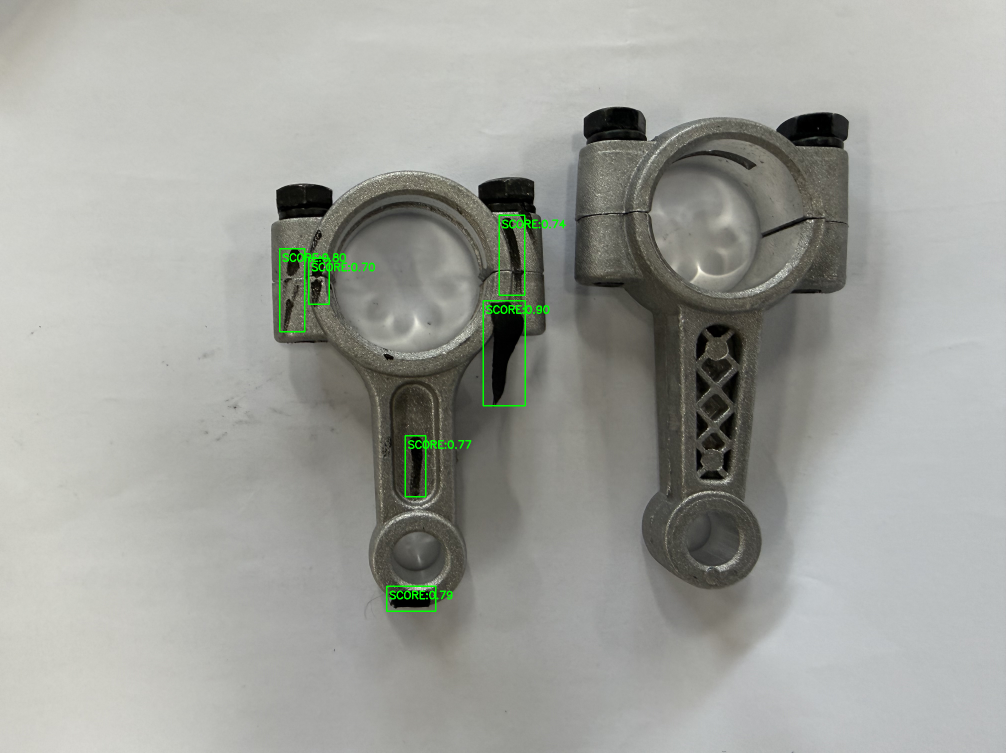
\includegraphics[width=0.7\textwidth]{result.png}
\caption{表面缺陷检测示例}\label{fig:defect_examples}
\end{figure}
在边缘侧部署 \textbf{LWDetr} 与 \textbf{GraspNet} 模型,实现对现场数据的实时处理:


\begin{itemize}
    \item \textbf{LWDetr 模型:}  
    基于 Transformer 架构的轻量级目标检测网络,通过特征金字塔和自注意力机制,在保持高检测精度的同时显著降低计算量,可在 Jetson AGX Orin 等嵌入式平台上实现实时推理,用于检测泵头零件表面的划痕与脏污。

    \item \textbf{GraspNet 模型:}  
    基于点云输入的深度抓取预测网络,通过并行卷积与姿态回归模块,直接输出三维抓取位姿(位置 + 姿态 + 抓取置信度),实现复杂堆叠场景下的无序抓取。

    \item \textbf{本地优化:}  
    推理端集成 TensorRT 加速与 INT8 量化,以实现高吞吐率和低延迟,满足生产线节拍需求。
\end{itemize}

\subsection{云端智能层:多模态大模型与 MCP 服务}

云端部署多模态工业大模型,作为系统的智能中枢,通过 \textbf{MCP} 与边缘节点进行数据交互与知识协同,主要功能包括:
% 请在您的 LaTeX 文档导言区确保包含以下宏包
% \usepackage{tikz}
% \usetikzlibrary{shapes.geometric, arrows.meta, positioning, fit}


\begin{itemize}
    \item \textbf{多模态数据理解:}  
    云端大模型可对边缘上传的图像、点云及日志信息进行联合分析,实现缺陷类型判别、异常样本聚类、以及检测模型自动再训练。

    \item \textbf{MCP 服务机制:}  
    MCP 提供标准化的任务通信接口(RESTful API / ROS2 Bridge),可动态下发检测参数、优化模型权重,并支持在线微调与模型版本管理。

    \item \textbf{知识增强决策:}  
    云端模型结合历史生产数据与知识图谱,对检测结果进行语义理解与趋势分析,从而对设备状态、产品质量给出预测性维护与调度优化建议。
\end{itemize}

\subsection{人机协同层:智能交互与多模态可视化}

本系统的人机协同层通过集成云端大语言模型(LLM)与多模态-控制-规划(MCP)服务接口,实现了对机械臂行为的直接自然语言控制。如图~\ref{fig:speech_to_action_pipeline_revised}所示,为确保交互的实时性与精确性,我们设计并实现了一条严谨的\textbf{流式语音到操作(Speech-to-Action)的交互逻辑链路}。
\begin{figure}[htbp]
    \centering
    % 使用 resizebox 将图表宽度强制缩放到与文本宽度一致,高度按比例自动调整
    % 这是解决 Overfull \hbox 警告最专业、最有效的方法
    \resizebox{\textwidth}{!}{
        \begin{tikzpicture}[
            node distance=1.5cm and 1.5cm,
            % --- 样式定义 ---
            block/.style={rectangle, draw, thick, rounded corners=3pt, fill=blue!10,
                          text width=2.5cm, minimum height=1.5cm, align=center, font=\small},
            io/.style={trapezium, trapezium left angle=70, trapezium right angle=110,
                       draw, thick, fill=green!15, minimum height=1.5cm, align=center, font=\small},
            data/.style={rectangle, draw, thin, fill=gray!10, font=\scriptsize\ttfamily, align=left, text width=4.5cm},
            feedback/.style={rectangle, draw, thick, rounded corners=3pt, fill=orange!10,
                             text width=4cm, minimum height=1.2cm, align=center, font=\small},
            line/.style={draw, -{Stealth[length=6pt,width=6pt]}, thick, shorten >=2pt, shorten <=2pt}
        ]
    
        % --- 节点定义 ---
        \node[io] (operator) {语音输入};
        \node[block, right=of operator] (asr) {
            \textbf{实时语音转录} \\ (ASR \& VAD)
        };
        \node[block, right=of asr] (llm) {
            \textbf{意图识别与指令生成} \\ (Instruction-Tuned LLM)
        };
        \node[block, right=2.5cm of llm] (mcp) {
            \textbf{指令校验与API转译} \\ (MCP 服务接口)
        };
        \node[io, below=2.5cm of mcp] (robot) {机械臂执行};
    
        % JSON指令节点
        \node[data, below=1cm of llm] (json) {
            \{ \\
            \quad "command": "set\_parameter", \\
            \quad "target": "joint", "id": 5, \\
            \quad "parameter": "max\_velocity", \\
            \quad "value": 30, "unit": "deg/s" \\
            \}
        };
    
        % 反馈闭环节点
        \node[feedback, below=of json, yshift=-1.5cm] (feedback) {
            \textbf{多模态可视化界面} \\ 实时参数更新 \& 语音确认
        };
    
        % --- 连线定义 ---
        \path[line] (operator.east) -- node[midway, above, font=\scriptsize] {语音流} (asr.west);
        \path[line] (asr.east) -- node[midway, above, font=\scriptsize] {转录文本} (llm.west);
        \path[line] (mcp.south) -- node[midway, above, font=\scriptsize] {底层API调用} (robot.north);
        \path[line] (llm.south) -- node[midway, left, font=\scriptsize, align=center] {结构化\\JSON指令} (json.north);
        \path[line] (json) -- (mcp);
        \path[line, orange!80!black]  (mcp.east) -- ++(2,0)  % 向右
  -- ++(0,-8)            % 向下
  -- (feedback.east);      % 向左连接到 feedback.east

        \path[line, orange!80!black] (feedback.west) -- (operator.south) node[pos=0.25, right, font=\scriptsize, black] {闭环反馈};
    
        % 整体模块虚线框
        \node[draw, dashed, inner sep=10pt, fit=(asr) (llm) (mcp), label={[font=\small\bfseries]above:Speech-to-Action 交互逻辑链路}] (pipeline) {};
    
        \end{tikzpicture}
    } % resizebox 命令的结束括号
    \caption{人机协同层的流式语音到操作(Speech-to-Action)交互逻辑链路}
    \label{fig:speech_to_action_pipeline_revised}
\end{figure}

该链路的工作流程如下:
\begin{enumerate}
    \item \textbf{实时语音转录与端点检测:} 前端麦克风阵列采集操作员的语音流,并实时传送至自动语音识别(ASR)服务。该服务采用流式识别模式,在操作员说话的同时即开始逐字生成文本,而非等待整句话结束后再处理。同时,语音活动检测(VAD)算法监测语音能量,一旦判断对话结束,立即将完整的转录文本发送至下一步。这一机制是实现低延迟交互的关键。

    \item \textbf{意图识别与结构化指令生成:} 转录文本被输入到经过特定指令微调(Instruction-Tuning)的大语言模型中。LLM的核心任务并非进行开放式对话,而是执行\textbf{意图识别}与\textbf{参数提取}。它将自然语言指令(如“将关节5的转速限制在每秒30度以内”)解析,并将其转换为一个预定义的、严格的\textbf{JSON格式结构化指令},例如:
        \begin{verbatim}
{
  "command": "set_parameter",
  "target": "joint",
  "id": 5,
  "parameter": "max_velocity",
  "value": 30,
  "unit": "deg/s"
}
    \end{verbatim}

    \item \textbf{指令校验与底层API转译:} 该JSON对象被发送至本地的MCP服务接口。MCP作为\textbf{安全中间件},首先对指令进行合法性与安全性校验(例如,检查设定值是否在机械臂的安全运动范围内)。校验通过后,MCP负责将该结构化指令精确地转译为机器人控制器能够执行的底层API调用或脚本命令,并下发给机械臂执行。
\end{enumerate}

整个交互过程通过多模态可视化界面进行闭环反馈。当指令被成功执行后,界面上的相关参数会实时更新,并伴有简短的语音确认(如“检测置信度已更新”),确保操作员对机器人的状态有完全、即时的掌控。这种将LLM的理解能力与MCP的精确控制相结合的架构,有效解决了从模糊的人类语言到精确的机器语言之间的转换鸿沟,极大地提升了复杂机器人系统的现场调试与人机协作效率。
% 请确保您的 LaTeX 导言区已加载以下库:
% \usepackage{tikz}
% \usetikzlibrary{shapes.geometric, arrows.meta, positioning, fit}

% 请确保您的 LaTeX 导言区已加载以下库:
% \usepackage{graphicx} % resizebox 功能需要此宏包
% \usepackage{tikz}
% \usetikzlibrary{shapes.geometric, arrows.meta, positioning, fit}





\subsection{系统数据流与云边协同示意}

如图~\ref{fig:cloud_edge_architecture} 所示,系统在检测、分析、反馈三个阶段实现边缘实时响应与云端智能决策的协同工作。

\begin{figure}[h]
    \centering
    \begin{tikzpicture}[
        node distance=2.2cm,
        block/.style={rectangle, draw, rounded corners, text centered, minimum height=1cm, minimum width=3cm, fill=gray!10},
        line/.style={draw, -{Stealth[length=6pt,width=6pt]}, thick, shorten >=1.5pt, shorten <=1.5pt}
    ]

    % nodes
    \node[block] (camera) {工业相机 / 点云采集};
    \node[block, right=of camera] (edge) {\shortstack{边缘计算节点\\(LWDetr + GraspNet)}};
    \node[block, below=of edge, yshift=0.15cm] (cloud) {\shortstack{云端多模态大模型\\+ MCP 协同服务}};
    \node[block, below=of camera] (ui) {人机交互终端};

    % lines
    \path[line] (camera.east) -- (edge.west) node[midway, above]{实时检测};
    \path[line] (edge.south) -- (cloud.north) node[midway, left]{数据上传 / 参数同步};
    \path[line] (cloud.west) -- (ui.east) node[midway, below]{多模态交互};
    \path[line] (ui.north) --(camera.south) node[midway, left]{指令下发 / 调度控制};

    \end{tikzpicture}
    \caption{云-边协同与多模态人机交互架构示意图}
    \label{fig:cloud_edge_architecture}
\end{figure}

通过上述架构,系统实现了:
\begin{itemize}
    \item 边缘侧的高效实时推理;
    \item 云端侧的知识增强与全局优化;
    \item 多模态交互的人机智能协同;
    \item 模型的自进化与持续优化。
\end{itemize}

\subsection{无序抓取模块设计}

在智能制造场景中,零件通常以无序堆叠方式放置在料框或传送带上,其姿态多变、部分遮挡严重,传统基于几何模板或规则匹配的方法难以满足实时性与鲁棒性要求。为此,本项目采用 \textbf{GraspNet} 深度学习抓取网络,实现无序环境下的三维抓取位姿预测与动作规划。

\begin{figure}[htbp]\centering
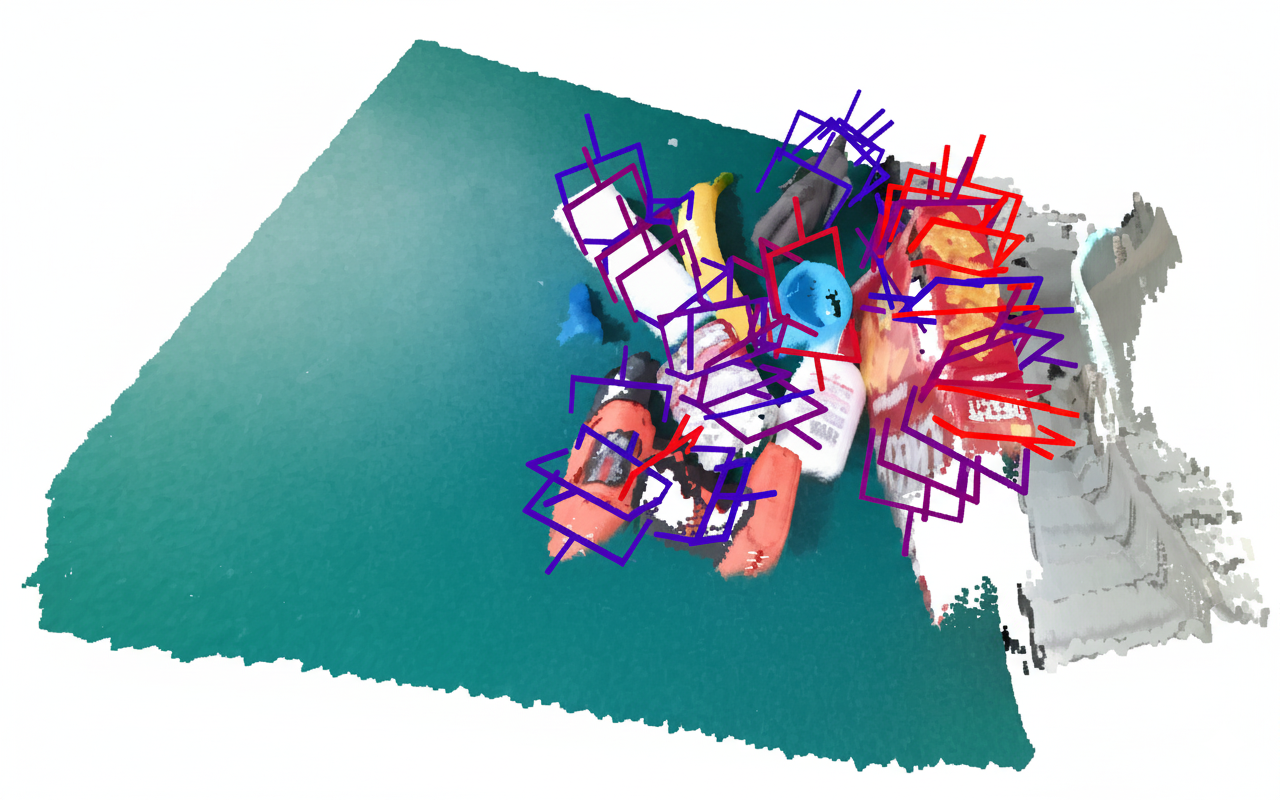
\includegraphics[width=0.7\textwidth]{graspnet.png}
\caption{GraspNet 抓取姿态可视化}\label{fig:grasp_viz}
\end{figure}
\subsubsection{网络结构与输入输出}

GraspNet 以点云数据为主要输入,核心结构包括:
\begin{itemize}
    \item \textbf{点云特征编码模块:} 采用 PointNet++ \cite{qi2017pointnet++} 或 SparseConv3D 提取空间局部特征,获得零件表面的几何描述;
    \item \textbf{候选抓取点生成模块:} 基于几何中心与表面法向分布,生成多组潜在抓取姿态;
    \item \textbf{抓取质量评估网络:} 通过卷积与注意力机制,预测每个候选姿态的抓取置信度(grasp quality score);
    \item \textbf{姿态回归模块:} 输出抓取位姿的六维参数 $\{x, y, z, \theta, \phi, \psi\}$,用于机械臂轨迹规划。
\end{itemize}

\subsubsection{点云采集与预处理}

\begin{itemize}
    \item 使用 RGB-D 相机或结构光传感器获取料框中零件的彩色与深度信息;
    \item 通过背景差分与 RANSAC 平面去除算法,剔除料框底面及噪声点;
    \item 采用体素下采样(Voxel Grid)与法线估计,生成高质量输入点云;
    \item 对检测出的缺陷区域附加语义标记,使抓取模块在规划时自动避开表面损伤部位。
\end{itemize}

\subsubsection{抓取推理与执行流程}

\begin{enumerate}
    \item 边缘端实时接收 \textbf{LWDetr} 的检测结果及位姿信息;
    \item 结合深度图生成对应的点云区域;
    \item 将点云输入 \textbf{GraspNet} 模型,获得抓取候选集与置信度;
    \item 选取置信度最高的候选抓取姿态;
    \item 通过机械臂控制模块调用逆运动学求解器(IK Solver),生成抓取轨迹;
    \item 执行抓取动作,并实时反馈执行状态至云端。
\end{enumerate}

\subsubsection{优化与云边协同}

\begin{itemize}
    \item \textbf{实时优化:} 边缘侧采用 TensorRT 部署 GraspNet,并利用局部点云裁剪与批处理推理,单帧推理延迟低于 60\,ms;
    \item \textbf{云端协同:} MCP 服务收集各抓取任务的执行数据,通过云端大模型对失败抓取样本进行再训练与姿态聚类,从而持续提升模型稳定性;
    \item \textbf{视觉-语义融合:} 通过多模态大模型对检测与抓取结果进行联合理解,实现“检测—抓取—分拣”决策的一体化。
\end{itemize}

通过上述设计,GraspNet 模块能够在复杂堆叠、光照变化及部分遮挡环境下实现高精度抓取预测,使系统具备真正的柔性生产与自适应分拣能力。


\section{创新点与实用性分析}

本项目面向智能制造场景下的零件检测与无序分拣任务,融合轻量化视觉检测、点云抓取网络、云边协同与多模态人机交互技术,构建高效、灵活、可扩展的智能系统,具有显著的创新性与实际应用价值。

\subsection{创新点}

\begin{enumerate}
    \item 轻量化检测与部署优化:采用改进的 LWDetr 作为缺陷检测核心,通过剪枝、蒸馏与 INT8 量化并结合 TensorRT 加速,在嵌入式与通用 GPU 平台实现高精度、低延迟的实时推理(检测延迟可低至 50\,ms)。优化的 anchor-free 结构更适应零件形状复杂、尺寸差异显著的检测任务,显著降低硬件成本。
    \item GraspNet 无序抓取与分拣策略:基于点云的深度抓取网络从单帧或多视角融合点云中直接预测最优 6D 抓取位姿,并输出抓取置信度;与检测语义融合后可自动避开受损区域。结合 ROS 2 \cite{quigley2009ros} 与 MoveIt\cite{sucan2012open} 的轨迹规划,兼顾精度与安全性。
    \begin{itemize}
        \item 零件姿态无关抓取:支持随机堆叠与部分遮挡场景的稳定抓取;
        \item 自适应抓取优化:依据表面法向与摩擦特性动态调整抓取姿态;
        \item 多物体分拣规划:将检测类别映射至不同目标位,实现自动上料与分类。
    \end{itemize}
    \item 云边协同的智能优化机制:通过 MCP 实现边缘实时检测与云端知识增强的双向交互。云端多模态模型可进行异常样本聚类、错误分析、在线微调与模型版本管理,并结合历史数据与知识图谱提供预测性维护与调度优化建议。
    \item 多模态人机协作交互:支持语音、文本、图像等多模态交互。操作人员可通过自然语言下达任务与参数变更,系统以图形化结果与语音播报反馈检测与分拣状态,提升交互效率与可解释性。
    \item 柔性化与模块化系统设计:基于 ROS 2 的模块化架构,采用标准化通信接口,便于与不同品牌的机械臂、传感器及生产管理系统集成,具备良好可扩展性,可推广至更多类型零件的检测与装配任务。
\end{enumerate}

\subsection{实用性与落地分析}

本系统在设计之初便充分考量了工业环境下的实用性与落地可行性。在硬件层面,我们选用 Jetson Orin NX 与 RealSense D455 等高性价比组合,确保方案能够经济、稳定地在单台工业机械臂上运行,其超越行业基准的抓取成功率可直接满足中小型制造企业对效率与成本的双重诉求。这不仅能通过自动化检测与分拣显著减少人工工作量,更能有效提升产线整体的良品率与生产节拍,带来直接的经济效益。

系统的核心优势更体现在其高度的灵活性与智能性。检测、抓取、分拣与交互等功能模块均可独立部署或联合运行,使其能快速迁移至不同生产线,并通过更换模型迅速适配新零件类型,展现了卓越的可扩展性。同时,我们引入的云端持续学习与在线微调机制,使系统具备了在不同批次与型号变化中自我优化的能力,极大降低了传统方案所需的人工标注与重新训练成本。

在保障层面,我们采用本地—云端分布式架构,确保核心数据在边缘端加密处理与推理,云端仅接收抽象特征用于模型迭代,有力地保障了企业生产信息的安全。

综上所述,该系统通用的架构与算法不仅解决了当前的应用难题,更具备向装配、搬运等更广泛工业环节推广的巨大潜力,为构建高柔性、可自优化的未来智能工厂提供了坚实的技术验证与可行的落地范例。

\begin{figure}[htbp]\centering
\fbox{\begin{minipage}[c][5cm][c]{0.9\linewidth}\centering 图占位:检测准确率/分拣成功率/节拍柱状图\end{minipage}}
\caption{性能指标对比(占位)}\label{fig:metrics}
\end{figure}

\section{总结与未来展望}

本项目以智能制造场景中的“三钢柱塞泵连杆配件原厂件泵头零件”为研究对象,针对零件表面划痕与脏污检测、复杂堆叠环境下的无序分拣问题,构建了一个集视觉检测、点云抓取、智能分拣与云端交互于一体的完整系统方案。

在系统架构上,采用 \textbf{LWDetr} 作为轻量化检测核心,兼顾高精度与实时性;在抓取策略上,引入 \textbf{GraspNet} 实现点云层面的稳定抓取;在系统集成层面,融合了 \textbf{本地轻量化模型 + 云端大模型 + MCP 多模态服务} 的协同架构,使得人机交互与任务调度更加自然与高效。整个方案具备可扩展、可迁移、低成本与高鲁棒性的特点,能够在典型制造业生产线上快速落地。

未来工作将围绕以下几个方向展开:

\begin{itemize}
    \item \textbf{强化学习优化抓取策略:} 结合深度强化学习框架(如 PPO、SAC)实现自适应抓取动作优化,使机器人能够在不同堆叠密度与摩擦环境下学习最优策略。
    \item \textbf{多模态协同感知:} 在视觉与力觉的基础上,融合声学与触觉信息,提升异常检测与抓取失败自恢复能力。
    \item \textbf{云端知识增强:} 通过与云端大模型持续联动,实现基于历史任务数据的知识蒸馏与在线模型重训练,形成“终身学习型”生产系统。
    \item \textbf{通用工业应用拓展:} 将本系统推广至齿轮、阀体、泵芯等多类零部件的检测与分拣场景,支持跨品类适配与视觉快速重构。
\end{itemize}

综上所述,本项目方案通过深度结合机器视觉、点云智能、云边协同与人机交互技术,为智能制造中的零件检测与无序分拣提供了一种高效、智能、具备落地潜力的解决路径,为未来工业生产的智能化升级提供了参考价值。
\newpage
\bibliographystyle{ieeetr}    % 或模板要求的样式
\bibliography{refs}

\end{document}




